\chapter{Visual Mobile Marker Odometry}
\label{chap:Visual Mobile Marker Odometry}


Visual pose estimation and localization is very important not only for robotic applications but also useful for augmented reality. Through camera configuration(monocular,
stereoscopic or multi-camera) in different environment as well as the amount of cognition about the structure and geometry of the environment 
we can find relatively reliable solutions to this problem.

A mobile multi-robot system which was firstly introduced in \cite{kurazume1994cooperative}
can obviously speed-up and improve the accuracy of the localization
of each of the robots. In this case, the concept of \textbf{Visual Mobile Marker Odometry}(\textbf{MOMA}) was proposed with the idea of cooperative positioning for multiple robots\cite{acuna2017moma}. 
%Visual Mobile Marker Odometry

Visual pose estimation can be divided into two different categories:

\begin{enumerate}
\item Marker-based(\textbf{MA}): using some detectable visual landmarks such as fiducial markers or 3D scene models with known coordinates of its features/keypoints\cite{acuna2017moma}. 
\item Markerless(\textbf{MAL}): based on static scene features with unknown absolute coordinates in the scene(without any knowledges of 3D scene).
\end{enumerate}

In figure \ref{fig:ma_mal} are shown both cases of pose estimation.
\begin{figure}[H]
\centering
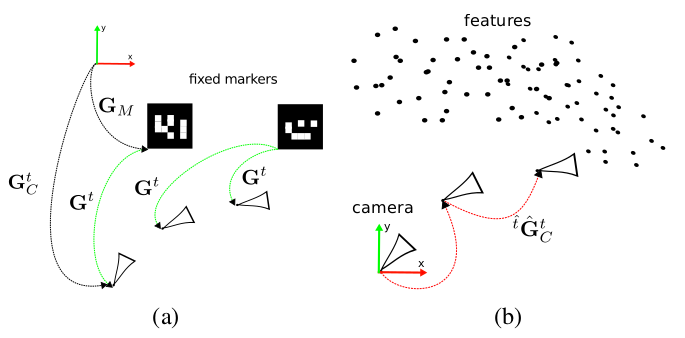
\includegraphics[scale=0.5]{./fig/ma_mal.png}
\caption{Marker-based(\textbf{MA}) pose estimation and markerless environment(\textbf{MAL-VO}) pose estimation\cite{acuna2017moma}.} 
\label{fig:ma_mal}
\end{figure}

Following we make a comparison of marker-based method and markerless method in some aspects: 
\begin{center}
   \begin{tabular}{ | l | p{5cm} | p{5cm} |}
    \hline
      & Pros & Cons\\ \hline 
    MA & not drift; reduce error from 3D to 2D only on image plane; relatively higher accuracy and lower computational complexity & require artificial markers in the environment \\ \hline
    MAL & without modification of artificial marker; can be used to detect real-world objects  & unavoidable drift; additional errors; need enough brightness and contrast of the environment   \\ \hline
    \end{tabular}
\end{center}


For our current work we only considered the case of marker-based(\textbf{MA}) method and we did the future work based on \textbf{MOMA} with two-robot caterpillar: one robot is carried with camera(monocular) as observer and the other robot is set with fiducial marker(\textbf{MA}).

The robot with camera and the robot with marker both have two states:

\begin{itemize}
\item \textbf{Mobile}: the robot is moving or permitted to move.
\item \textbf{Static}: otherwise.
\end{itemize}

The motion pattern for two-robot caterpillar is shown in figure \ref{fig:moma}. This is the background of our simulation scene.

\begin{figure}[h]
\centering
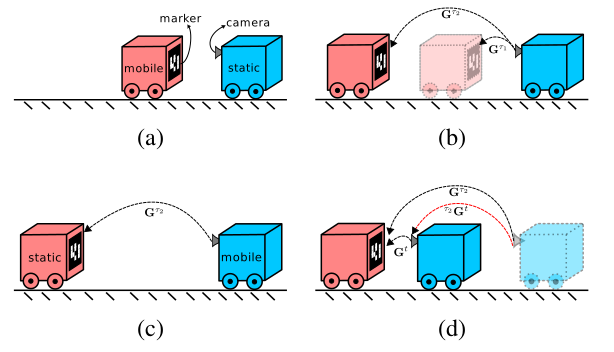
\includegraphics[scale=0.5]{./fig/moma.png}
\caption{Two-robot caterpillar. At the beginning, the robot with camera is static and the robot with marker is mobile. And then, the marker and camera exchange states which means move in turns, now the camera is mobile and marker is static. Finally, we can get the pose estimation between them\cite{acuna2017moma}.}
\label{fig:moma}
\end{figure}
